


\subsection{Recent results}

The Kamioka Liquid Scintillator Anti-Neutrino Detectro (KamLAND) was 
designed as search for the oscillation of electron antineutrinos
emitted from nuclear power stations. 
Typical baseline of 180~km intended to adress the oscillation
solution to the ``solar neutrino problem''.
Use inverse $\beta~\text{-decay}$ to detect electron
antineutrinos. 1~kton ultrapure LS detector.
2003, first evidence of electron antineutrino disappearance. Ratio of 
observed inverse $\beta-\text{decay}$ events to expected events
without electron neutrino disappearance
was $0.611 \pm 0.085\text{(stat.)} \pm
0.041\text{(syst.)}$. Fewer events than expected at the 99.95\%
confidence level.~\cite{Kamland:PhysRevLett.90.021802}  
2005, direct evidence for neutrino oscillations via observation of 
distortion in rector electron antineutrino energy
spectrum.~\cite{Kamland:PhysRevLett.94.081801} 
More rectently in 2008. 
Exposure of $2.44 \times 10^{32} \text{proton yr}$
Measured values: 
$\Delta m^2_{21} =
7.58^{+0.14}_{-0.13}\text{(stat.)}^{+0.10}_{-0.06}\text{(syst.)}$  and
$\tan^2\theta_{12} =
0.56^{+0.10}_{-0.07}\text{(stat.)}^{+0.10}_{-0.06}
\text{(syst.)}$.~\cite{Kamland:PhysRevLett.100.221803}  

The Sudbury Neutrino Observatory (SNO) was created to measure the flux
of neutrinos produced in the Sun, by $^8$B decays in particular.
1~kton detector. Imaging Cherenkov detector using
heavy water($^2\text{H}_2\text{O}$. 1.783~km below sea level and an 
overburden of 5.890~km water equivalent. SNO detected neutrinos via 
three processes: elastic scattering, charged current and neutral
current interactions. Measuring the rates of these three processes
gave insight on the overall flux of neutrinos from the sun and also
the flux of electron neutrinos that reach the
detector. By comparing these fluxes SNO was able to test the neutrino
oscillation hypothesis.~\cite{SNO:PhysRevC.81.055504}   
In 2013. Combined result of SNO and all other solar and reactor
neutrino experiments gave
$\Delta m^2_{21} = (7.46^{+0.20}_{-0.19}) \times 10^{-5}~eV^2$, 
$\tan^2\theta_{12} = 0.443^{+0.030}_{-0.025}$ and 
$\sin^2\theta_{13} = (2.49^{+0.20}_{-0.32}) \times
10^{-2}$.~\cite{SNO:PhysRevC.88.025501}  


The Super Kamiokande (SK) is an imaging water Cherenkov detector
designed to detect neutrinos produced by $^8$B decays in the Sun.
2011 paper. Solar neutrino experiment measuring flux of electron
neutrinos from the sun from the stellar production of nuetrinos from
the $^8$B reaction chain. Via neutrino electron scattering. Located
1~km underground. 50~ktons of ultrapure water. signals read out ny
photomulilyer tubes.
Three flavour fit produces
$\sin^2\theta_{12} = 0.30 ^{+0.02}_{-0.01}$ and $\Delta m^2_{21} = 6.2
^{+1.1}_{-1.9} \times 10^{-5}~eV^2$.  In combination with other solar
experiments and KamLand found $\sin^2\theta_{13} =
0.025^{+0.018}_{-0.016}$.~\cite{SK:PhysRevD.73.112001}~\cite{SK:PhysRevD.83.052010} 
%~\cite{SK:PhysRevD.73.112001, SK:PhysRevD.83.052010}


Measurement of electron antineutrino disappearance with the Daya Bay
experiment. Non zero value of $\theta_{13}$ measured with precision by
Daya Bay, which measured $\sin^22\theta_{13} = 0.084 \pm 0.005$.  
Total exposure of $6.9 \times 10^5~\text{GW}_{th}$~ton~days.
Opening the door to the measurement of electron neutrino 
apearance in a muon neutrino beam and hence measurements of the mass 
hierarchy and the cp violating phase $\delta_{CP}$.
Fully constructed experiment consists of 8 detectors and 6 nuclear
reactor cores.~\cite{DayaBay-PhysRevLett.115.111802}
Large value of $\sin^2\theta_{13}$ measured by Daya Bay \cite{DayaBay2012}.

RENO is a reactor antineutrino disappearance experiment. Reactor
electron antineutrinos are detected via inverse
$\beta$~decay. Conincidence of prompt positron signal and a delayed
photon signal from neutron capture is the signature for inverse $\beta$~decay.
Two identical detectors located 
294~m and 1383~m from the centre of six reactor
cores. Each detector consists of a main inner detector and an outer
veto detector.$\sin^22\theta_{13} = 0.082 \pm 0.009(\text{stat.}) \pm
0.006(\text{syst.})$. \cite{RENO:2015ksa}~\cite{RENO:PhysRevLett.108.191802}

The Double Chooz experiment measures reactor antineutrino
disappearance. 
Far detector is located at an average distance of 1050~m from the two
reactor cores at the Chooz nuclear power plant. 
Measured: 
$\sin^22\theta_{13} = 0.090^{+0.032}_{-0.029}$.~\cite{Abe:2014bwa}   

%MINOS
The Main Injector Neutrino Oscillation Search (MINOS) experiment was
designed to measure the flavour composition of a muon neutrino beam at 
two locations using a near and far detector located 1~km and 735~km
from the target respectively. 
In 2006 the first muon neutrino
disappearance results observed 215~events compared to an expectation
of $336 \pm 14~\text{events}$ and were consistent with disappearance
via oscillations.~\cite{MINOS:PhysRevLett.97.191801}
Most recently, in 2015 a joint analysis of accelerator and atmospheric
neutrinos combining muon neutrino
disappearance, electron neutrino apearance further improved the
precision of parameter measurements with the results 
$|\Delta m^2_{32} = |2.28-2.46| \times 10^{-3}~eV^2$
~\cite{MINOS:PhysRevLett.112.191801} 


%T2K

%NOvA

\section{Weak Interactions}

Neutrinos interact with matter via the weak force mediated by the W
and Z bosons.

\section{Neutrino Eigenstates}

As current understanding has it, neutrinos come in three eigenstates
of the weak force (electron, muon and tau) and three mass eigenstates
($m_1$, $m_2$ or $m_3$).  

Neutrinos interact with matter through the weak force in eigenstates
of lepton flavour ($\nu_e$, $\nu_{\mu}$ and $\nu_{\tau}$). They
propagate through vacuum in eigenstates of mass ($\nu_1$, $\nu_2$ and
$\nu_3$). The eigenstates of mass and flavour are not equivalent,
instead the flavour states are a superposition of the mass states.  
A neutrino of definite weak flavour $\alpha$ can be written as a
linear combination of the mass states as follows, 

\begin{equation}
|\nu_{\alpha}> = \sum_{i=1}^{3} U^{*}_{\alpha i}|\nu_i>,
\end{equation}

\noindent where $U^* _{\alpha i}$ is the element of the unitary PMNS
(Pontecorvo, Maki, Nakagawa, and Sakata) matrix describing the
coupling strength between the mass state $i$ and the flavour state
$\alpha$.  

The standard parametrisation of the PMNS matrix is in terms of a phase
$\delta$ and three mixing angles, $\theta_{12}$, $\theta_{13}$ and
$\theta_{23}$. The PMNS matrix is conventionally written as: 

\begin{align}
  U &= 
      \begin{pmatrix}
        U_{e1} & U_{e2} & U_{e3} \\
        U_{\mu 1} & U_{\mu 2} & U_{\mu 3} \\ 
        U_{\tau 1} & U_{\tau 2} & U_{\tau 3}
      \end{pmatrix}\\
    &=
      \begin{pmatrix}
        c_{13}c_{12} & c_{13}s_{12} & s_{13}e^{-i\delta} \\
        -c_{23}s_{12}-s_{13}s_{23}c_{12}e^{i\delta} &
        c_{23}c_{12}-s_{13}s_{23}s_{12}e^{i\delta} & c_{13}s_{23} \\ 
        s_{23}s_{12}-s_{13}c_{23}c_{12}e^{i\delta} &
        -s_{23}c_{12}-s_{13}c_{23}s_{12}e^{i\delta} & c_{13}c_{23} 
      \end{pmatrix}\\
    &=
      \begin{pmatrix}
        1 & 0 & 0 \\
        0 & c_{23} & s_{23} \\
        0 & -s_{23} & c_{23} 
      \end{pmatrix}
                      \begin{pmatrix}
                        c_{13}             & 0 & s_{13}e^{-i\delta} \\
                        0                  & 1 & 0                  \\
                        -s_{13}e^{i\delta} & 0 & c_{13}
                      \end{pmatrix}
                                                 \begin{pmatrix}
                                                   c_{12}  & s_{12} & 0 \\
                                                   -s_{12} & c_{12} & 0 \\
                                                   0       & 0      & 1
                                                 \end{pmatrix}
\label{eqn:PMNS}
\end{align}

\noindent where $s_{ij} \equiv \sin\theta_{ij}$, $c_{ij} \equiv
\cos\theta_{ij}$ and $\delta$ is the CP violating phase. A non-zero
value of $\delta$ would indicate charge-parity violation.



\section{Neutrino Oscillation Probability in Vacuum}

The following derivation of the neutrino oscillation probability
follows~\cite{pdg}~and~\cite{Hiroshi}.

A neutrino is produced via a weak interaction as a flavour
eigenstate. At time $t=0$ the flavour state, $\alpha$, can be written
as $|\nu_{\alpha}\left(t=0\right)>$ and is the sum of the mass states
$|\nu_i>$: 

\begin{equation}
|\nu_{\alpha}\left(t=0\right)> = \sum_{i=1}^{3} U^{*}_{\alpha i}|\nu_i>.
\label{eqn:sumAtTime0}
\end{equation}

% The neutrino mass states time-evolve according to the Sch{\"o}dinger
% equation: 
% \begin{equation}
% i\dfrac{d}{dt}|\nu_i(t)> = \mathcal{H}|\nu_i(t)>,
% \label{eqn:schrodinger}
% \end{equation}

% \noindent with eigenvalues $E_i$. The mass states can be described as a plane wave:
% \begin{equation}
% |\nu_i(t)> = e^{-iE_{i}t}|\nu_i>.
% \label{eqn:timeEvolveMassStates}
% \end{equation}

% Using Equations~\ref{eqn:sumAtTime0}~and~\ref{eqn:timeEvolveMassStates} gives:
% \begin{equation}
% |\nu_{\alpha}(t)> = \sum_{i=1}^{3} U^{*}_{\alpha i} e^{-iE_{i}t}|\nu_i>.
% \end{equation}

As the neutrino propagates the mass states evolve. At time t we have: 
\begin{equation}
|\nu_{\alpha}\left(t\right)> = \sum_{i=1}^{3} U^{*}_{\alpha i}
e^{-ip_i.x}|\nu_i>, 
\end{equation}
\noindent where $p_i$ is the four-momentum and $x$ the four-position
of mass state $\nu_i$. 

% At time t the neutrino interacts with matter through the weak
% force. The wavefunction is collapsed into a weak eigenstate
% $<\nu_{\beta}| = \sum_{j=1}^{3} U_{\beta j}<\nu_j|$. We have: 
At time t the neutrino weakly interacts with matter in flavour state $\beta$:

\begin{equation}
\begin{split}
<\nu_{\beta}|\nu_{\alpha}> &= \sum_{j=1}^{3}\sum_{i=1}^{3}U_{\beta j}
U^{*}_{\alpha i} e^{-ip_i.x} <\nu_j|\nu_i>\\ 
&= \sum_{j=1}^{3}U_{\beta j}   U^{*}_{\alpha j} e^{-ip_j.x}.
\end{split}
\label{eqn:nubeta_nualpha}
\end{equation}

Assuming all mass states have the same three-momentum \textbf{p}, 

\begin{equation}
  \begin{split}
    p_j.x & = E_jt - \textbf{p} \cdot \textbf{x} \\
    & =t\sqrt{|\textbf{p}|^2 + m_j^2} - \textbf{p} \cdot \textbf{x}
  \end{split}
\end{equation}

Since neutrinos are extremely light ($m_{\nu} < 2~eV$ \cite{pdg}) and,
in the case of accelerator experiments, travel at close to the speed
of light we can make the approximations, $m_j << E_j$, $t = L$ and $
\textbf{p} \cdot \textbf{x} = |\textbf{p}|L$. Using a binomial
expansion we find,  

\begin{equation}
p_j \cdot x = |\textbf{p}|L\left( 1 + \dfrac{m_i^2}{2|\textbf{p}|^2 }
\right) - |\textbf{p}|L  = \dfrac{m_jL}{2E}
 \label{eqn:binomialExp}
\end{equation}


Combining Equations~\ref{eqn:nubeta_nualpha}~and~\ref{eqn:binomialExp}
we get $<\nu_{\beta}|\nu_{\alpha}> = \sum_{j=1}^{3}U_{\beta j}
U^{*}_{\alpha j} e^{-i\dfrac{m_jL}{2E}}$. 

The probability of observing the neutrino in flavour state $\beta$
after travelling distance $L$ and given initial flavour state $\alpha$
is given by: 

\begin{equation}
\begin{split}
P_{\alpha \rightarrow \beta} & = |<\nu_{\beta}\left(t\right) |
\nu_{\alpha}\left(t\right)>|^2\\ 
& = \left( \sum_{j=1}^{3}U_{\beta j}   U^{*}_{\alpha j}
  e^{-i\dfrac{m_jL}{2E}}\right) 
\left(\sum_{i=1}^{3}U^*_{\beta i}   U_{\alpha i}
  e^{i\dfrac{m_jL}{2E}}\right). 
\end{split}
\end{equation}

Finally, we find:

\begin{equation}
\begin{split}
P_{\alpha \rightarrow \beta} = \delta_{\alpha \beta}  
&- 4 \sum_{i>j}\mathfrak{R}[U^*_{\alpha i} U_{\alpha j} U_{\beta i}
U^*_{\beta j}] \sin^2\left(\dfrac{\Delta m^2_{ij}}{4E} L\right)\\ 
&+ 2 \sum_{i>j}\mathfrak{I}[U^*_{\alpha i} U_{\alpha j} U_{\beta i}
U^*_{\beta j}] \sin^2\left(\dfrac{\Delta m^2_{ij}}{2E} L\right), 
\end{split}
\label{eqn:genTransProb}
\end{equation}

\noindent where $\Delta m^2_{ij} \equiv m^2_i - m^2_j$ and
$\delta_{\alpha \beta}$ is the Kronecker delta. The equation shows
that the neutrino oscillation probability depends on the parameters of
the PMNS matrix and the value of 
% $\sin^2\left(\dfrac{\Delta
%   m^2_{ij}}{4E} L\right)$
the two sinusoidal arguments.
The probability depends on the mass
splittings $\Delta m_{12}^2$,  $\Delta m_{13}^2$,  $\Delta m_{23}^2$,
and alters with the length of the baseline, L, and the energy of the
neutrino beam, E.  

\section{Neutrino Oscillation Paremeter Measurements}

The experimentally measured values of the neutrino oscillation
parameters are given in Table~\ref{tab:paremeterValues}. The
measurements of the oscillation parameters have been made using
reactor, solar, accelerator and atmospheric neutrino
experiments. 
% reactor neutrino results
% accelerator neutrino results
% limits on neutrino mass

% mass ordering
The two mass differences and three mixing angles have all been
measured. The sign of the mass difference has been determined for
$\Delta m^2_{12}$ ($\nu_1$ is less massive than $\nu_2$) but not for
$\Delta m^2_{23}$. This means that it is not known whether $\nu_3$ is
more or less massive than the two other mass states, the former and
later cases are known as Normal Ordering or Inverted Ordering
respectively. A schematic showing the Normal and Inverted Ordering is
shown in Figure

% cp violation
Tentative measurements of the CP violating phase $\delta_{CP}$ have
been made \cite{FA_nue} but the value remains relatively unknown. 

% octant
Current measurements suggest that $\sin^2\theta_{23} = 0.5$ which
would mean $\cos^2\theta_{23} = 0.5$. In this case,
$U_{\mu2} = U_{\tau3} = \dfrac{1}{2}c_{13}$ (see
Equation~\ref{eqn:PMNS}). These two PMNS matrix elements define the
mixing of $\nu_{\mu}$ and $\nu_{\tau}$ with $\nu_3$. Therefore, if
$\sin^2\theta_{23} = 0.5$ then the third mass state is composed of
equal parts $\nu_{\mu}$ and $\nu_\tau$, this is known as maximal
mixing. If nature has chosen non-maximal mixing then discovering the
octant (whether $\sin^2\theta_{23}$ is less or more than 0.5) will
determine whether the third mass state is composed of more $\nu_\mu$
or more $\nu_\tau$. 

\begin{table}
  \centering
  \begin{tabular}{ l | l  }
    \hline
    Parameter & Average of measurements \\ \hline
    $\sin^2 \theta_{12}$  & 0.304 $\pm$ 0.014 \\
    $\Delta m^2_{21} ~[10^{-5}~\text{eV}^2]$  & 7.53 $\pm$ 0.18 \\
    $\sin^2\theta_{23}$   & 0.51 $\pm$ 0.05 (0.50 $\pm$ 0.05)  \\
    $\Delta m^2_{32} ~[10^{-3}~\text{eV}^2]$ & 2.44 $\pm$ 0.06 (-2.51 $\pm$ 0.06)\\
    $\sin^2\theta_{13} ~[10^{-2}]$ & 2.19 $\pm$ 0.12 \\
    \hline
  \end{tabular}
  \caption{
    The average value of measurements and 1$\sigma$ error of
    the neutrino oscillation parameters from
  \cite{pdg}. Measurements that differ under the assumption of
  inverted ordering (rather than normal ordering) are provided
  within parenthesis.} 
  \label{tab:paremeterValues}
\end{table}



\section{Two-Flavour Approximation}

In many experimental cases the neutrino oscillation probability can be
approximated as the result of two-flavour mixing. This two flavour
oscillation probability and the necessary approximation will be
outlined in this section.

For long baseline neutrino oscillation experiments it is useful to
write the phase $\dfrac{\Delta m^2_{ij}}{4E} L$ in units of the same
scale as the experiment. This is done using units of $\text{eV}^2$ for
$\Delta m^2_{i}$, GeV for $E$ and km for $L$. Restoring factors of
$\hbar$ and $c$ and applying the appropriate unit conversions we find: 
\begin{equation}
\dfrac{\Delta m^2_{ij}c^3}{4E\hbar} L \approx 1.27 \dfrac{\Delta
  m^2_{ij} [\text{eV}^2]}{E [\text{GeV}]} L [\text{km}].
\end{equation}

Let us use the oscillation channel relevant to this thesis as the
example. In the three flavour case (Equation~\ref{eqn:genTransProb}),
the muon neutrino survival probability is:
\begin{equation}
P_{\mu \rightarrow \mu} = 1
- 4 \sum_{i>j}
|U_{\mu i}|^2 |U_{\mu j}|^2 
\sin^2\left(\dfrac{\Delta m^2_{ij}}{4E} L\right),
\end{equation}
\noindent where the imaginary component of
Equation~\ref{eqn:genTransProb} is zero because in this case 
$\mathfrak{I}[U^*_{\mu i} U_{\mu i}] = 0$.

The elements of the PMNS matrix, $U_{\mu i}$, can be simplified
considering the current measured values.
Table~\ref{tab:paremeterValues} shows that the value of
$\sin^2\theta_{13}$ is very small relative to the two other mixing
parameters. Using the approximations $\sin\theta_{13} \approx 0$
and $\cos\theta_{13} \approx 1$ the relevant PMNS elements (see
Equation~\ref{eqn:PMNS} can be approximated as:

\begin{equation}
\begin{aligned}
&|U_{\mu 1}|^2  \approx s_{12}^2c_{23}^2 \\
&|U_{\mu 2}|^2  \approx c_{12}^2c_{23}^2 \\
&|U_{\mu 3}|^2  \approx s_{23}^2
\end{aligned}
\label{eqn:simpleficationMatrixElements}
\end{equation}


Experimental results have shown that the mass splitting $\Delta
m_{12}^2$ is very small relative to $\Delta m_{13}^2$ and $\Delta
m_{23}^2$ (see Table~\ref{tab:paremeterValues}) \cite{pdg}, which
allows the approximation: $\Delta m_{13}^2 \simeq \Delta
m_{23}^2$. 
For long baseline neutrino oscillation experiments the
oscillations associated with the atmospheric and solar mass splittings
can be approximated to be de-coupled. This is because the atmospheric
mass splitting is $\sim$30 times larger than the solar mass splitting.  
As an example, let us take the NOvA experiment with $L =
810~\text{km}$ and $E \sim 2~\text{GeV}$. For the NOvA experiment the
we have:
\begin{equation}
\sin^2\left(\dfrac{1.27 \Delta m^2_{12}}{E} L \right) = \sin^2
\left(\dfrac{1.27 \times 7.53 \times 10^{-5}}{2} \times 810 \right)
\approx \sin^20.04 \approx 0.
\end{equation}

With the above simplifications, the muon neutrino survival probability
can be expressed as:
\begin{equation}
  \begin{aligned}
    P_{\mu \rightarrow \mu} 
    &\simeq 1 - 4 s_{23}^2c_{23}^2(s_{12}^2 + c_{12}^2) \sin^2 \left(
      \dfrac{1.27\Delta m_{atm.}^2}{E} L \right)\\  
    &\simeq 1 - \sin^22\theta_{23}\sin^2 \left( \dfrac{1.27\Delta
        m_{atm.}^2}{E} L  \right),  
  \end{aligned}
\end{equation}
\noindent where $\Delta m^2_{atm.} \equiv \Delta m^2_{32} \simeq
\Delta m^2_{13}$. From this equation it can be seen that the
disappearance probability has an oscillatory form. The overall
magnitude of the oscillation is governed by $\sin^22\theta_{23}$ and
the period of the oscillation is defined by $\dfrac{\Delta m_{atm.}^2 L}{E}$.


% The large mass splitting, $\Delta m_{23}^2$ or $\Delta
% m_{13}^2$, is known as the atmospheric mass splitting and the small
% mass splitting, $\Delta m_{12}^2$, is known as the solar mass
% splitting. 






\section{Matter Effects}

Neutrinos propagating through matter experience the weak force through
NC interactions and coherent forward scattering. Ordinary matter is
composed, in part, of electrons but not muons or taus. For this reason
coherent forward scattering (shown in Figure~\ref{diag:CohForScat}) is
only experienced by electron neutrinos. In addition, NC interactions
with matter are flavour independant and so do not affect neutrino
oscillations. 
This additional scattering amplitude causes oscillations involving
$\nu_e$ or $\bar{\nu}_e$ to have different probabilities relative to
oscillation in vacuum.

% Cite the papers \cite{Mikheyev1986} and \cite{WolfensteinMatter}

\begin{figure}[h]
  \centering
  \begin{fmffile}{diagram}
    \begin{fmfgraph*}(200,100)
      \fmfleft{i1,i2} \fmfright{o1,o2}
      \fmf{fermion}{i1,v1,o1} \fmf{fermion}{i2,v2,o2}
      \fmf{dashes,label=$W$}{v1,v2} \fmfdot{v1,v2}
      \fmflabel{$e$}{i1}
      \fmflabel{$\nu_e$}{i2}
      \fmflabel{$\nu_e$}{o1}
      \fmflabel{$e$}{o2}
    \end{fmfgraph*}
  \end{fmffile}
  \caption{Feynman diagram of coherent forward scattering of $\nu_e$
    on $e$.}
  \label{diag:CohForScat}
\end{figure}

The evolution of the neutrino flavour states is given by
\begin{equation}
 i\dfrac{d}{dx} \left( 
   \begin{array}{c}
     \nu_e\\
     \nu_\mu\\
     \nu_\tau
   \end{array}
   \right) =
   H \left(
   \begin{array}{c}
     \nu_e\\
     \nu_\mu\\
     \nu_\tau
   \end{array}
   \right),
\end{equation}
\noindent where $H$ is the Hamiltonian. In matter $H$ is given by
\begin{equation}
  H = U
  \begin{pmatrix}
    \dfrac{m_1^2}{2E} & 0 & 0 \\
    0 & \dfrac{m_2^2}{2E} & 0 \\ 
    0 & 0 & \dfrac{m_3^2}{2E}
  \end{pmatrix}
  U^\dagger +
  \begin{pmatrix}
    \sqrt{2}G_FN_e & 0 & 0 \\
    0 & 0 & 0 \\ 
    0 & 0 & 0
  \end{pmatrix},
\end{equation}
\noindent where $G_F$ is the Fermi constant and $N_e$ is the electron
number density of the medium. 

Matter effects modify the terms
$\sin \left( \Delta_{31} \right)$ and $\sin\left( \Delta_{21}
\right)$ (where $\Delta_{ij} \equiv \dfrac{\Delta m_{ij}^2}{4E}L$)in
Equation~\ref{eqn:genTransProb} by substituting: 

\begin{equation}
\sin \left( \Delta_{ij} \right) \rightarrow
\dfrac{\Delta_{ij}}{\Delta_{ij} \mp aL} 
\sin \left( \Delta_{ij} \mp aL \right),
\end{equation}
\noindent where $a = \dfrac{G_F\rho_e}{\sqrt{2}}$, the top sign refers
to neutrinos and the bottom sign to antineutrinos. \cite{TDR} 

For the Normal Ordering, matter effects enhance the apearance
probability $\nu_\mu \rightarrow \nu_e$ but suppress the apearance
probability $\bar{\nu}_\mu \rightarrow \bar{\nu}_e$. Conversely, for
the Inverted Ordering matter effects suppress the $\nu_e$ apearance
probability and enhance the $\bar{\nu}_e$ probability.

% bi-probability plot
Matter effects have the opposite consequence for neutrinos and
antineutrinos and so can be confused with the effect of true CP
violation. Figure~\ref{fig:BiProb} illustrates the ambiguity between
CP and matter effects when measuring the neutrino and antineutrino
apearance. 
The figure shows regions of bi-probability where it is possible to
disentangle the contributions of matter effects and CP violation. In
particular, for the inverted hierarchy and $\delta_{CP} = 3\pi /2$
(the starred point) NOvA would be able to measure the mass ordering to 
be Normal with some confidence. This point would correspond to
measured probabilities of $P(\bar{\nu}_e) = 0.025$ and $P(\nu_e) =
0.06$. 
Conversely, if NOvA measures $P(\bar{\nu}_e) = 0.04$ and $P(\nu_e) =
0.04$ then it will not be possible to distinguish between two possible
scenarios: either the ordering is normal and $\delta_{CP} \approx \pi
\ 2$ or the ordering is inverted and $\delta_{CP} \approx 3 \pi
\ 2$.
The two elipses shown are for fixed values of 
$\sin^2\left( 2\theta_{13} \right)$, $\sin^2\left( 2\theta_{23}
\right)$ and $\Delta m_{32}^2$. The effect of increasing (decreasing)
$\theta_{23}$ is to increase (decrease) both apearance probabilities
and make the ellipses less (more) ambiguous.

\begin{figure}
  \centering
  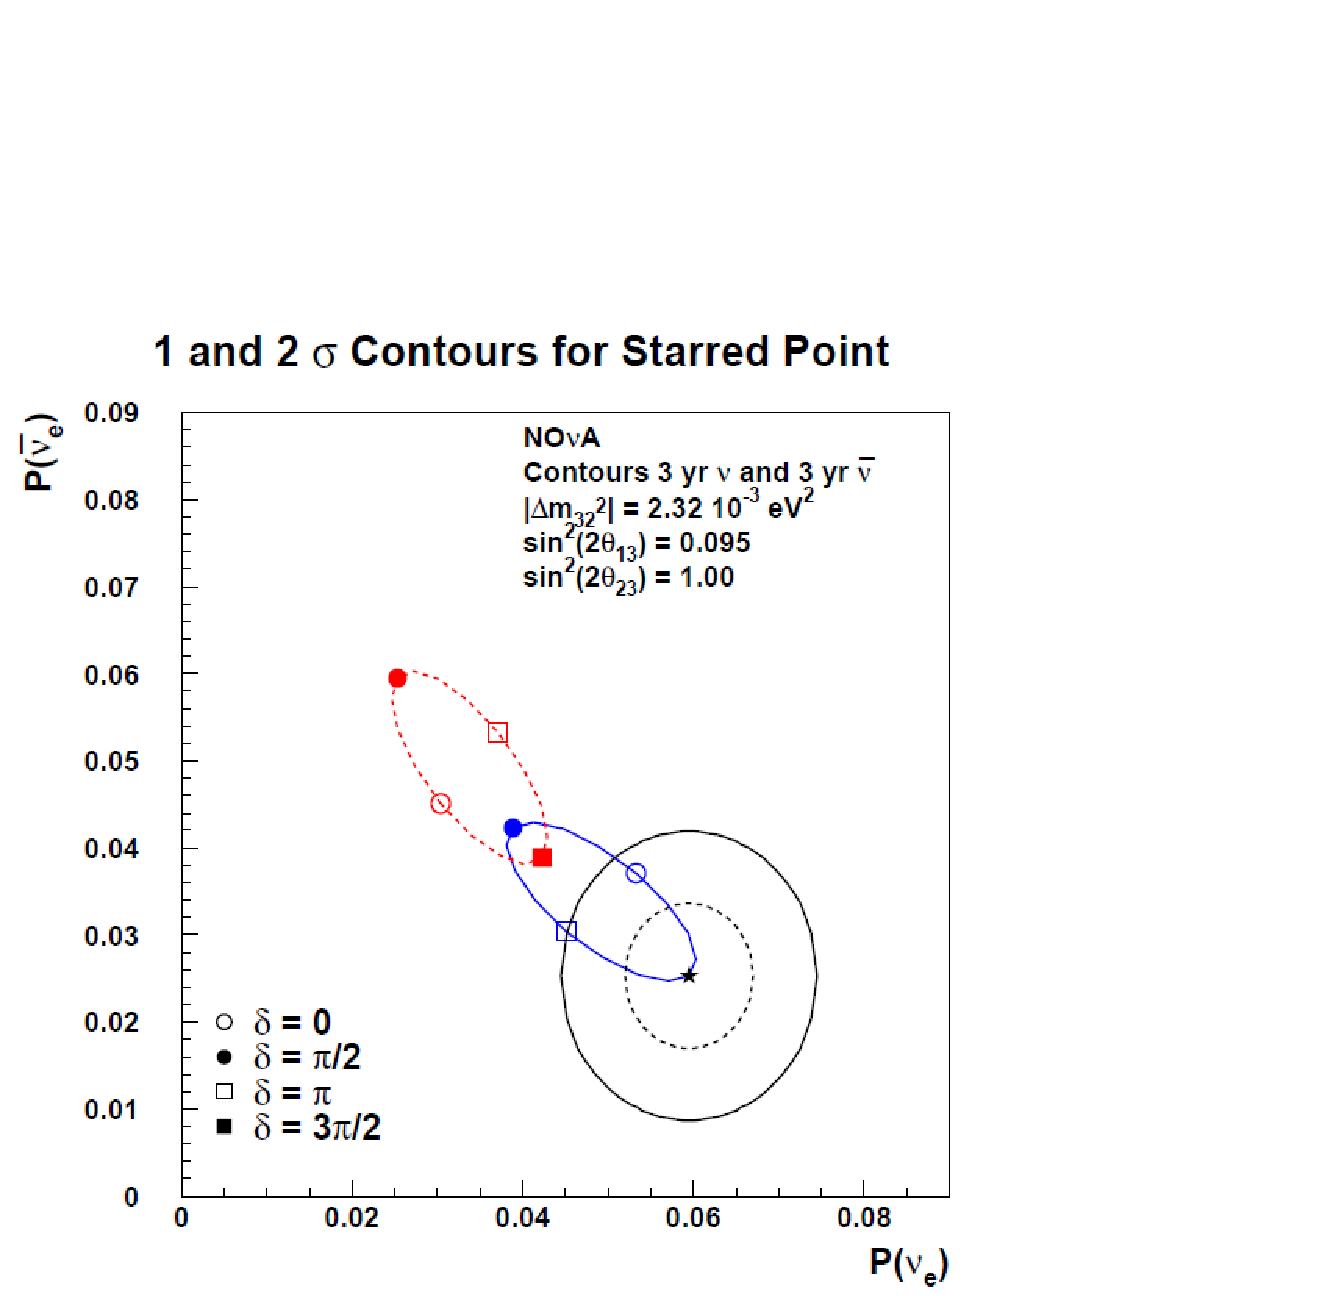
\includegraphics[width=0.9\textwidth]{../../img/Theory/09_Bi-Probability_Plots.pdf}
  \caption{
    Bi-probability plot of $\nu_e$ apearance for the NOvA experiment. 
    The solid blue and dotted red elipses show the possible
    probability measurements for the Normal and Inverted Ordering
    respectively. The effect of altering $\delta_{CP}$ is to trace out the
    ellipse. Selected values of $\delta_{CP}$ are shown by the square
    and circle markers.
  } 
  \label{fig:BiProb}
\end{figure}